\documentclass[a4paper]{article}
\usepackage{iwslt15,amssymb,amsmath,epsfig,subfig,adjustbox}
\usepackage{siunitx, diagbox}
\usepackage{hyperref}
\usepackage{tikz}
\setcounter{page}{1}
\sloppy		% better line breaks
%\ninept
%SM below a registered trademark definition
\def\reg{{\rm\ooalign{\hfil
     \raise.07ex\hbox{\scriptsize R}\hfil\crcr\mathhexbox20D}}}

%% \newcommand{\reg}{\textsuperscript{\textcircled{\textsc r}}}

\title{Digit String Recognition}

%%%%%%%%%%%%%%%%%%%%%%%%%%%%%%%%%%%%%%%%%%%%%%%%%%%%%%%%%%%%%%%%%%%%%%%%%%
%% Please make sure to keep technical paper submissions anonymous  !
%%%%%%%%%%%%%%%%%%%%%%%%%%%%%%%%%%%%%%%%%%%%%%%%%%%%%%%%%%%%%%%%%%%%%%%%%%
%\name{Firstname Lastname}
%%%%%%%%%%%%%%%%%%%%%%%%%%%%%%%%%%%%%%%%%%%%%%%%%%%%%%%%%%%%%%%%%%%%%%%%%%
%% If multiple authors, uncomment and edit the lines shown below.       %%
%% Note that each line must be emphasized {\em } by itself.             %%
%% (by Stephen Martucci, author of spconf.sty).                         %%
%%%%%%%%%%%%%%%%%%%%%%%%%%%%%%%%%%%%%%%%%%%%%%%%%%%%%%%%%%%%%%%%%%%%%%%%%%
\makeatletter
\def\name#1{\gdef\@name{#1\\}}
\makeatother
\name{{\em Lucas Steinmann, Leandro Piekarski, Hesham Hendy,}\\
      {\em Manuel Olk}}
%%%%%%%%%%%%%%% End of required multiple authors changes %%%%%%%%%%%%%%%%%

\address{Praktikum Neuronale Netze  \\Karlsruhe Institute of Technology, Germany \\
%{\small \tt firstname.lastname@iwslt.org}
}
%
\begin{document}
\maketitle
%
\begin{abstract} \label{sec:abstract}
Convolutional Neural Networks have been widely used in recent years as powerful feature extractors to solve different computer vision tasks. Combined with Connectional Temporal Classification it is possible to train end-to-end models to be successful in tasks which involve both feature extraction from images and sequence labeling such as digit string recognition. This work reimplements a previously proposed CNN + RNN-CTC network and evaluates it on the datasets provided for the HDSRC2014 competition. By combining data from different datasets, recognition rates on ORAND-CAR-A, ORAND-CAR-B and CVL of 91.27\%, 94.08\% and 75.79\% are achieved respectively. In addition to it, the performance impact of the RNN part of the network is evaluated. 

\end{abstract}


%
\section{Introduction} \label{introduction}
In recent years the recognition of handwritten digits has been systematically improved. Benchmarked on the MNIST (Mixed National Institute of Standards and Technology)
dataset that contains about 70.000 images of handwritten digits along with their corresponding labels, numerous papers were published that apply convolutional neural networks (CNNs)
to achieve error rates of 0.23\% \cite{MNIST_2012} or even 0.21\% \cite{MNIST_boosting}.

As these results almost cope with human performance and a good dataset does need to represent a sufficiently challenging problem to stay useful and to ensure its longevity, various adjustments can be contemplated. One way could be the extension of the underlying dataset \cite{EMNIST}.

Another approach would be the extension of the task itself by not only recognizing single digits but whole digit strings. In 2014 the ICFHR (International Conference on Frontiers in Handwriting Recognition) announced a competition to attend that matter: Handwritten Digit String Recognition in Challenging Datasets (HDSRC2014) \cite{icfhr_competition}.

In course of that they proposed a new benchmark framework that consists of two real world datasets and respective evaluation measures. The task's complexity is not only founded on the connected digits but also on the additional challenges that come along with the images' real world nature as document layout, background texture or noisy strokes. 

Traditional approaches to digit string recognition often used segmentation. The string image is segmented to pieces that in best case represent single digits. The recognition results of these single pieces are then combined to get global optimal results. Since these approaches in practice suffer from various handwritten styles, connected or even overlapped characters and noises, \cite{zhan2017} proposes an segmentation free approach. 

Their model uses ResNet with convolutional layers \cite{ResNet} as an discriminative sequence extractor and feature decoder, combines it with an bidirectional LSTM and calculates the loss with connectionist temporal classificiation (CTC) \cite{CTC}.

Since this approach achieved remarkable results on the given datasets we used it as fundament for our own model.

The rest of this paper is organized as follows. In Section 2 we briefly describe the real world datasets given by the HDSRC2014. ...... Then, details of our experiments are presented in Section 3. Section 4 concludes this paper and discusses potential future work.

\section{Databases} \label{Datasets}
There are two different databases for recognizing handwritten digit strings we used in our experiments.

The first database, named ORAND-CAR, is a real world database with 11719 images of the 'Courtesy Amount Recognition (CAR)' field of bank checks. It originates from two different sources, one bank of Chile and one of Uruguay, and therefore shows different characteristics in terms of check layout, image quality and further noise. That is the reason the database is splitted into two subsets called ORAND-CAR-A (CAR-A) and ORAND-CAR-B (CAR-B). Samples of both datasets are shown in Figure \ref{fig:carA} and \ref{fig:carB}.

\begin{figure}
  \includegraphics[width=\linewidth]{images/CAR-A-Splitted.png}
  \caption{Sample images of ORAND-CAR-A}
  \label{fig:carA}
\end{figure}

\begin{figure}
  \includegraphics[width=\linewidth]{images/CAR-B-Splitted.png}
  \caption{Sample images of ORAND-CAR-B}
  \label{fig:carB}
\end{figure}

CAR-A's training set consists of 2009 images whereas the testing set delivers 3784 images. In CAR-B there are 3000 training images and 2926 images for testing.

The second database we worked on is called Computer Vision Lab Handwritten Digit String (CVL HDS). It contains handwritten digits of 300 different writers without any background noise. The training set includes only 10 different digit strings from about 125 writers which leads to an overall amount of 1262 images for training. In the testing set we have the same 10 digit strings from the remaining writers and 16 new strings from all 300 writers to reach 6698 testing images. CVL HDS provides us with large variability with respect to handwriting styles but lacks diversity in the digit strings themselves. Examples of the CVL HDS database are shown in Figure \ref{fig:cvl}.

\begin{figure}
  \includegraphics[width=\linewidth]{images/CVL-HDS-Splitted.png}
  \caption{Sample images of CVL HDS}
  \label{fig:cvl}
\end{figure}

The datasets differ with respect to their string lengths. CVL has images with string lengths from 5 to 7 whereas CAR-B offers digit strings from length 4 to 8. In this regard CAR-A comes with the biggest variety and covers a string length range from 2 to 8 digits. A summary of the string length distribution can be seen in Table \ref{table_string_lengths}.

\begin{table}
\caption{\label{table_string_lengths} {\it Summary of string length distribution.}}
\vspace{2mm}
\hspace{1mm}
\begin{adjustbox}{width=0.45\textwidth}
\centerline{
\begin{tabular}{|l|lll|lll|}
\hline
\multicolumn{1}{|l|}{} & & Training & & & Testing & \multicolumn{1}{l|}{}\\
\multicolumn{1}{|l|}{len} & \multicolumn{1}{l|}{CAR-A} & \multicolumn{1}{l|}{CAR-B} & \multicolumn{1}{l|}{CVL} & \multicolumn{1}{l|}{CAR-A} & \multicolumn{1}{l|}{CAR-B} & \multicolumn{1}{l|}{CVL} \\ \hline
2 & 22 & 0 & 0 & 36 & 0 & 0  \\
3 & 204 & 0 & 0 & 387 & 5 & 0  \\
4 & 704 & 63 & 0 & 1425 & 69 & 0  \\
5 & 903 & 1200 & 125 & 1475 & 1241 & 789  \\
6 & 145 & 1599 & 758 & 363 & 1452 & 4144  \\
7 & 29 & 137 & 379 & 87 & 157 & 1765  \\
8 & 2 & 1 & 0 & 11 & 2 & 0  \\
\hline
$\Sigma$ & 2009 & 3000 & 1262 & 3784 & 2926 & 6698  \\
\hline
\end{tabular}}
\end{adjustbox}
\end{table}

Since the images of the used databases come in lots of different aspect ratios and we want them to fit our model, we resize them to a fixed width of 120 and an height of 50.

 We furthermore make use of the different tools given by Pytorch to augment our data. Dynamic data augmentation is achieved with help of the functions ColorJitter() and RandomAffine(). How the data is transformed, can be seen in Figure \ref{fig:dataAug}.

\begin{figure}
  \includegraphics[width=\linewidth]{images/Data-Augmentation.png}
  \caption{Examples of an image after preprocessing and data augmentation.}
  \label{fig:dataAug}
\end{figure}

\section{Connectionist Temporal Classification}\label{sec:ctc}

The Loss has been calculated using CTC. It can be considered as an output layer of Neural network to deal with the following main problems:
\begin{itemize}
%\itemsep -1.3mm
\item The consumed time during the annotation process of the whole data set on digit level, which would be one to one correspondence between outputs and labels.
\item The limitation on the available information about the digits and its constraints which could be affected during the processing through many factors like noise or image resolution.
\end{itemize}
So These issues can be avoided through a function which is provided with the output matrix of the NN and the corresponding ground-truth (GT) text by trying all possible digit alignments between inputs and labels in the image and outputs at the end a classification at each input value by taking the highest score which conclude the real value. CTC uses the network to label the entire input sequence at once. This means the network can be trained with an unsegmented data set, and the final label sequence can be seen directly from the network output. The input of CTC is a sequence $y=y_{1},....y_{T}$ from a recurrent neural network with m inputs and n outouts, where T is the sequence length, For instance for an input squence y of length T, definde a RNN with m inputs, n ouputs and weight vektor w as a continous map $N_w$: ($\mathbb{R^m}$) $\rightarrow$  ($\mathbb{R^n}$).Then the first step called Encoding can be initiated through inserting randomly a pseudo character called Blank denoted with {-} which must be inserted in case of digits duplication. For a given $y_{T}$ it gives us an output distribution over all possibilities.Then a conditional probability is defined as the sum of probabilities of all $\pi$ which are mapped by F onto I:
\begin{equation}
p( I | y)=\sum_{\pi \in F(I)} p( \pi | y )
\label{eq3}
\end{equation}
where the conditional probability of $\pi$ is defined as: 
\begin{equation}
p( \pi | y ) =\prod_t^T y_{\pi_{t}}
\label{eq3}
\end{equation}
The probability $p( \pi | y )$ of a particular path or respectively label observing is the product of all the softmax outputs "digit scores" $y_{\pi_{t}}$ over time T for one alignment. The function takes the negative log probability of ground truth all the training examples in training set D
\begin{equation}
\sum_{(i,y)_{\in D}} - \log  p( I | Y )
\label{eq3}
\end{equation}
where y is the sequence produced by the recurrent layers from x. Then we should update the network through back propagation. By decoding, the function calculates the best path by taking the most likely character per time-step and undoes the encoding measures by first removing duplicate characters and then removing all blanks from the path and as a result remains the recognized text \cite{CTC}.


\section{Recurrent Neural Network}\label{sec:rnn}
Based on the human fact that we do not need to rethink from scratch rather building up on the available results, Recurrent Neural Network has been developed to solve this issue with the normal neural network using connected chunks of neural network. The information can be passed over the chunks in a loop intimately, but It shouldn’t go so far back to avoid gradient vanish problem during the parameter optimization especially by a small number of Iterations. So LSTM should be used instead of the RNN.The LSTM short of learning long-term dependencies does have the ability to remove or add information to the cell state, carefully regulated by 4 specified mechanism called gates:
\begin{itemize}
%\itemsep -1.3mm
\item Forgetting mechanism.
\item Saving (remembering) mechanism.
\item Learning mechanism.
\item Focusing long-term memory into working memory which is the next short memory.
\end{itemize}
LSTM transforms its memory in a very precise way using these mechanisms for which pieces of information to remember, which to update, and which to learn. This helps it keep track of information over longer periods of time. At the same time, the future events should be also considered, therefore the network will be handle that trainings in the opposite direction, i.e each training sequence forwards and backwards to two separate LSTM layer, und that has been called bidirectional LSTM. 

\section{Approach}\label{sec:approach}

\subsection{Architecture}\label{subsec:architecture}
This section covers the architecture, with which we achieved our best results, which are presented in Section \ref{sec:evaluation}. Our architecture is based on a published architecture~\cite{CTC} which achieved the best performance in the competition ICFHR 2014~\cite{icfhr_competition}.

The task of digit string recognition poses several challenges across different machine learning disciplines.
On the one hand, the input image is a high-dimensional tensor (after resizing $120\times50\times3$).
As a consequence, the input will have a low information density and considerable amount of noise.
A proven neural network architecture class for processing images are convolutional neural networks (CNN).
More specifically, we employ a smaller variant of the Residual Network (ResNet)~\cite{ResNet} architecture.
See Fig.~\ref{fig:resblock} for a detailed view of our implementation of the residual architecture.
After every convolutional layer we performed batch normalization~\cite{batchnorm} to prevent internal covariance shift and accelerate training.
This first step in our architecture can be seen as an \emph{encoder}, mapping the input image to a 3 dimensional tensor with lower spatial dimensions ($15 \times 6$) but more channels (512).

We then interpret the output as a sequence along the horizontal axis.
For simplicity we have designed the horizontal output dimension of the encoder to be equal to the maximal sequence length.
In this case every column matrix (of size $6 \times 512$ represents one sequence element).
If this is not possible or the sequence length should be variable without changing the encoder, a linear projection can be used to increase or decrease the horizontal dimension.

The remaining task is to decode this tensor by labeling every element of the sequence with a digit or blank.
We output scores for every digit and blank for each element in the sequence.
The output dimensionality of every label is therefore 11.
The class network architecture we use for this task are called recurrent neural networks (RNNs).
As described in Section \ref{sec:rnn}, vanilla RNNs suffer from the vanishing gradient problem.
We therefore use long short term memory (LSTM)~\cite{LSTM}, which mitigate this issue.
LSTMs can be stacked by using the output of the previous layer as input to the next layer.
We use two layer LSTMs to allow the network to learn a more complex function.
In addition we use bidirectional LSTMs (BiLSTM), which are independently applied to the original sequence and the reversed sequence and combine their outputs by addition.
Our BiLSTM outputs a 100-d vector at every time step.
Finally a linear layer is used to reduce this dimension to 11.
During training we use log-softmax to prepare the output for calculation of the CTC-Loss.
When inferring labels we select the element with the highest output using the argmax operator at each time step.
The full architecture is shown in Fig.~\ref{fig:architecture}.

\begin{figure}
    \begin{center}
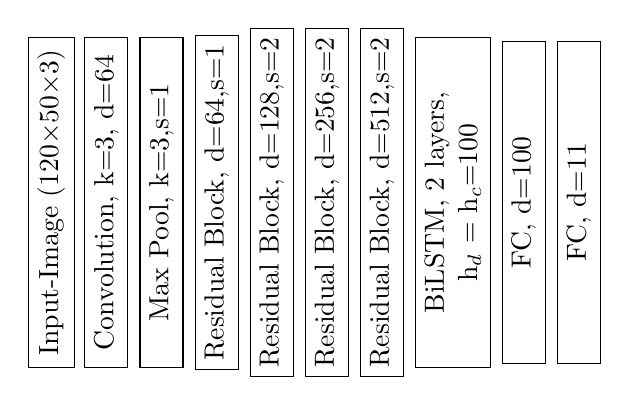
\begin{tikzpicture}
    \node[rectangle,minimum width=4.2cm,draw,rotate=90] at (0,2.1) (input) {Input-Image (120$\times$50$\times$3)};
    \node[rectangle,minimum width=4.2cm,draw,rotate=90] at (0.7,2.1) (conv1) {Convolution, k=3, d=64};
    \node[rectangle,minimum width=4.2cm,draw,rotate=90] at (1.4,2.1) (pool1) {Max Pool, k=3,s=1};
    \node[rectangle,minimum width=4.2cm,draw,rotate=90] at (2.1,2.1) (res1) {Residual Block, d=64,s=1};
    \node[rectangle,minimum width=4.2cm,draw,rotate=90] at (2.8,2.1) (res2) {Residual Block, d=128,s=2};
    \node[rectangle,minimum width=4.2cm,draw,rotate=90] at (3.5,2.1) (res3) {Residual Block, d=256,s=2};
    \node[rectangle,minimum width=4.2cm,draw,rotate=90] at (4.2,2.1) (res4) {Residual Block, d=512,s=2};
    %\node[rectangle,minimum width=2.1cm,draw,rotate=90] at (5.25,1.05) (reverse) {reverse};
    \node[rectangle,minimum width=4.2cm,draw,rotate=90,align=center] at (5.1,2.1) (bilstm) {BiLSTM, 2 layers, \\ $\text{h}_d$ = $\text{h}_c$=100};
    \node[rectangle,minimum width=4.1cm,draw,rotate=90] at (6,2.1) (fc1) {FC, d=100};
    \node[rectangle,minimum width=4.1cm,draw,rotate=90] at (6.7,2.1) (fc2) {FC, d=11};
\end{tikzpicture}
\caption{\it Schematic of our architecture. Dropouts and batch normalizations are omitted for brevity.}\label{fig:architecture}
\end{center}
\end{figure}
\begin{figure}
    \begin{center}
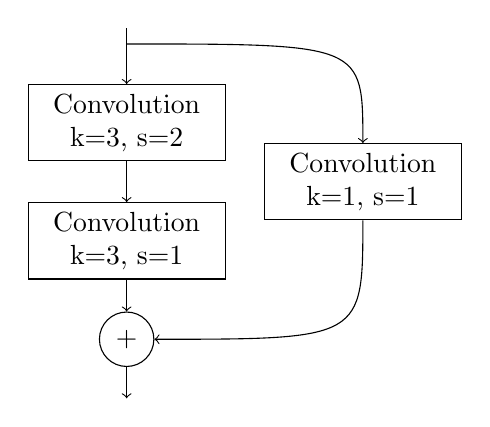
\begin{tikzpicture}
    \node[rectangle, minimum width=2.5cm,draw,align=center] at (0,-1) (conv1) {Convolution\\ k=3, s=2};
    \node[rectangle, minimum width=2.5cm,draw,align=center] at (0,-2.5) (conv2) {Convolution\\ k=3, s=1};
    \node[rectangle, minimum width=2.5cm,draw,align=center] at (3,-1.75) (resconv) {Convolution\\ k=1, s=1};
    \node[circle,draw,align=center] at (0,-3.75) (add) {$+$};
    \draw[->] (0,0.2) -- (conv1);
    \draw[->] (conv1) -- (conv2);
    \draw[->] (0,0) .. controls (3,0) .. (resconv);
    \draw[->] (conv2) -- (add);
    \draw[->] (resconv) .. controls (3,-3.75) .. (add);
    \draw[->] (add) -- (0,-4.5);
\end{tikzpicture}
\caption{\it Schematics of a residual block in our architecture. If the output dimension does not change (as in our first residual block, the linear mapping in the residual path is not required and therefore omitted. Furthermore does the first residual block use a stride of 1 instead of 2.}\label{fig:resblock}
\end{center}
\end{figure}
\subsection{Training}\label{subsec:training}

We divided our training in epochs.
In each epoch we observe every training sample once.
Each sample is randomly manipulated by different data augmentation methods as described in Section \ref{Datasets}.
We normalized each sample by channel-wise whitening (subtracting dataset mean color value and dividing by dataset variance).
The Adam~\cite{Adam} is used to minimize the CTC loss per batch.
We found a batch-size of 32 to deliver the best results.
Higher batch-sizes resulted into very slow learning, due to seldom updates, while lower batch-sizes did had less parallelization on GPU and where therefore slower to compute.
Increasing the step size when using higher batch-sizes did not speed up training either.
We suspect that the loss function surface is shaped in a way, such that higher variance gradient descent (as achieved by lower batch-sizes) results in faster convergence.

For hyper-parameter optimization we split our training data in a training and validation dataset, whereby 80\% of the training data is used for training and the rest is only used to evaluate the model performance.


\section{Evaluation}

\begin{table}
\caption{\label{table_zhan_interpretation} {\it Overall comparison between implementations.}}
\vspace{2mm}
\centerline{
\begin{tabular}{*{4}{|c}|}
\hline
Methods & 
CAR-A &
CAR-B & 
CVL\\
\hline \hline 
Zhan el al. 2017 & 0.8975 & 0.9114 & 0.2707 \\
Our "interpretation" & 0.9014 & 0.9084 & 0.2550 \\
\hline
\end{tabular}}
\end{table}

\begin{table}
\caption{\label{table_different_sets} {\it Performance on different sets.}}
\vspace{2mm}
\centerline{
\begin{tabular}{*{4}{|c}|}
\hline
Tested / Trained & 
CAR-A &
CAR-B & 
CVL\\
\hline \hline 
CAR-A & \textbf{0.9014} & 0.7315 & 0.002 \\
CAR-B & 0.8434 & \textbf{0.9084} & 0.006 \\
CVL & 0.3019 & \textbf{0.5804} & 0.2550 \\
\hline
\end{tabular}}
\end{table}

\begin{table}
\caption{\label{table_fine_tuning} {\it Performance using more than one set + fine tuning.}}
\vspace{2mm}
\centerline{
\begin{tabular}{*{3}{|c}|}
\hline
Tested / Trained & 
CAR-A + CAR-B &
CVL (fine tuning)\\
\hline \hline 
CAR-A & \textbf{0.9127} & 0.0565 \\
CAR-B & \textbf{0.9408} & 0.4733 \\
CVL & 0.5913 & \textbf{0.7579} \\
\hline
\end{tabular}}
\end{table}


\section{Conclusions}

This paper has described a novel approach for doing wonderful stuff such as ...

%
\bibliographystyle{IEEEtran}

%\begin{thebibliography}{10}
\bibitem[1]{ES1} Smith, J. O. and Abel, J. S., 
``Bark and {ERB} Bilinear Transforms'', 
IEEE Trans. Speech and Audio Proc., 7(6):697--708, 1999.  
\bibitem[2]{ES2} Lee, K.-F., Automatic Speech Recognition: 
The Development of the 
SPHINX SYSTEM, Kluwer Academic Publishers, Boston, 1989.
\bibitem[3]{ES3} Rudnicky, A. I., Polifroni, Thayer, E. H.,
 and Brennan, R. A.  
"Interactive problem solving with speech", J. Acoust. Soc. Amer., 
Vol. 84, 1988, p S213(A).
\end{thebibliography}
\bibliography{bib_}

\end{document}

